\documentclass[10pt, a4paper]{article}
\usepackage{float}
\usepackage{geometry}
\usepackage{listings}
\usepackage{pgfplots} 
\usepackage{hyperref}
\usepackage{graphicx}
\usepackage{ragged2e}
\usepackage{color}
\usepackage{xepersian}
\usepackage{subfiles}
\usepackage{multirow}
\usepackage{url}

\newgeometry{left=1.4cm, right=1.4cm, bottom=2.0cm, top=2.0cm}
\settextfont[Scale=1]{XB Roya}

\title{گزارش تحقیق شبکه تعاملی و فعل و انفعالات پروتئین‌ها}
\author{
    علیرضا سلطانی نشان \\
    گرایش مهندسی نرم‌افزار \\
    a.soltani@iau-tnb.ac.ir
  \and
    شقایق راجی \\
    گرایش مهندسی نرم‌افزار \\
    shaqayq.raji021@gmail.com
}

\begin{document}
\maketitle

\section*{چرایی این گزارش}

داده‌هایی که مربوط به روابط پروتئین‌ها در سطح اینترنت وجود دارد، داده‌هایی بسیار
ارزشمندی هستند که به ما در درمان بیماری‌های مختلف کمک خواهند کرد. وجود این
داده‌ها به ما این کمک را می‌کند که بتوانیم پیچیدگی بین مولکولی را کشف کنیم و
عملکرد آنها را بیاموزیم که بعد از آن بتوانیم با ترکیب آنها به پروتئین‌های جدیدی
برسیم که کاربرد‌های بسیار مهمی را در زندگی بشر ایفا می‌کنند.

منبع‌های بسیاری در این رابطه وجود دارد مانند \lr{ProBIS} \cite{konc2022protein}
که در مقاله \lr{Protein binding sites for drug design} که در نشریه \lr{Springer}
می‌توان آن را یافت، بسیار صحبت می‌کند. اما ما می‌توانیم از \lr{Api}های آزاد منبع
\lr{String} \footnote{ \lr{STRING is a database of known and predicted
protein-protein interactions. The interactions include direct (physical) and
indirect (functional) associations; they stem from computational prediction,
from knowledge transfer between organisms, and from interactions aggregated from
other (primary) databases.} } استفاده کنیم که داده‌های آن تا به امروز به بیشتر
از ۲۰ میلیون روابط پروتئین‌ها را دارا می‌باشد. در این بین بایستی اشاره کرد که در
دیتابیس‌های آن ۶۷,۵۹۲,۴۶۴ پروتئین را از ۱۴,۰۹۴ اورگانیسم پوشش می‌دهد.

در این گزارش سعی بر شناخت برخی پروتئین‌ها را داریم و علاوه‌بر آن سعی کردیم که
روابط بین پروتئین‌هایی که بعداً به آن‌ها اشاره‌ می‌کنیم را به وسیله ابزاری مناسب
به سریع‌ترین حالت ممکن در گراف نمایش دهیم تا شناخت و تشخیص آن‌ها را برای ما
ملموس کند.

\newpage
\tableofcontents
\newpage

\section{آشنایی قبلی}

\subsection{\lr{AlphaFold}}

\begin{figure}[H]
    \centering
    \includegraphics[width=0.5\textwidth]{images/sample_alphafold.png}
    \caption{نمونه‌ای از آلفافولد}
    \label{fig: alphafold}
\end{figure}

یک ابزار هوش مصنوعی معرفی شده توسط دیپ‌مایند گوگل است که به وسیله داده‌های
فراوانی که دارد می‌تواند ساختار سه بعدی پروتئین‌ها و آمینواسید‌ها را با دقت بالا
پیشبینی کند. استفاده از آن می‌تواند در موارد زیر بسیار مفید باشد:

\begin{itemize}
    \item درک بهتر عملکرد پروتئین‌ها و توابع آن‌ها
    \item طراحی دارو‌های جدید
    \item با استفاده از پیشبینی‌هایی که این ابزار انجام می‌دهد، تحلیل و مقایسه
    ساختاری پروتئین‌ها را برای متخصصین آسان می‌کند که از طریق آنها می‌توانند به
    دنبال الگو‌ها و تفاوت‌های مهم در ساختار باشند.
    \item سایر کاربرد‌های پزشکی و زیست شناسی 
\end{itemize}

\subsection{پروتئین‌ها}

اجزای اساسی مهم زندگی هستند. در تشکیل بسیاری از سلول‌ها، بافت‌ها و اعضای بدن
انسان و سایر موجودات زنده نقش بسیار مهمی دارند. ساختار و ویژگی هر پروتئین را
آمینواسید‌های آن مشخص می‌کند. (آمینواسید‌ها به صورت پیوسته به یکدیگر متصل
هستند). هر آمینواسید در یک زنجیره پروتئینی در یک نقطه از دایره می‌باشد. وقتی
نقاط را به هم وصل می‌کنیم، یک زنجیره خطی به وجود می‌آید که امکانات و قابلیت‌های
مختلفی دارد. این امکانات و قابلیت‌ها می‌توانند به عنوان ویژگی‌های پروتئین‌ها
تعریف شوند که رفتار آن‌ها را مشخص می‌کند. مانند \lr{Struct}هایی هستند که درون
آنها \lr{Trait}ها و ویژگی‌های مختلفی نوشته شده است.

طبق نوع و محل حضور پروتئین‌ها در عملکرد متفاوت هستند:

\begin{enumerate}
    \item فعالیت آنزیمی به منظور کاتالیز فرآیند
    \item شناسایی میکروب‌ها و سلول‌های سرطانی
    \item انتقال موادی مانند گاز‌های تنفسی و \underline{سیگنال‌دهی}
\end{enumerate}

\subsection{بسپار یا پلیمر}

یک درشت مولکول است که از تعداد انبوهی از اجزای کوچک‌تری به نام مونومر تشکیل شده
است، به گونه‌ای که زنجیره‌ای به هم متصل هستند(بس: بسیار، پار: پاره، قطعه).

پروتئین‌ها مانند زنجیره‌ای از یک کلافی سه بعدی از بسپار‌هایی هستند که از ترکیب
اسید‌های آمینه حاصل می‌شوند.

\subsection{اسید‌های آمینه}

اسید‌های آمینه یا آمینواسید‌ها ترکیبات آلی متشکل از گروه‌های عاملی آمینو و
کربوکسیلیک اسید هستند، بیشتر از ۵۰۰ آمینواسید در طبیعت وجود دارد. مهم‌ترین
امینواسید از نوع آلفا می‌باشد.

نکته: ۲۲ اسید آمینه آلفا واحد‌های تشکیل دهنده پروتئین هستند.

\section{روابط و پروتئین‌های بررسی شده}

\subsection{دادهای تحلیل شده}

مجموعه داده‌های ما شامل فعل و انفعالات جفتی برای تعداد انگشت شماری از پروتئین
هایی است که در مسیرهای سروتونین دخیل هستند.

\subsection{لیست پروتئین‌های مورد بررسی در این تحقیق}

\begin{table}[H]
    \centering
    \caption{پروتئین‌های بخش سروتونین}
    \begin{tabular}{c|c}
        نام پروتئین & کاربرد \\ \hline
        \lr{TPH1} & راهبرد در سنتز سروتونین \\
        \lr{TPH2} & کلیدی در تولید سروتونین: (تریپتوفان هیدروکسیلاز ۲) \\
        \lr{COMT} & تجزیه کاتکولامین‌ها: (کاتکول امینه ترانسفراز) \\
        \lr{SLC18A2} & حمل وستیکول‌های سروتونین: (پروتئین حمل‌کننده وستیکولر ۲ بخشی) \\
        \lr{SLC6A4} & حمل سروتونین از فضای سیناپسی: (پروتئین حمل‌کننده سروتونین) \\
        \lr{HTR1B} & نقش در تنظیم خواب و اضطراب: (گیرنده ۱ اسروتونین) \\
        \lr{HTR2C} & تاثیرگذاری بر اشتها و تغذیه: (گیرنده ۲ اسروتونین) \\
        \lr{HTR2A} & نقش در تنظیم خواب و شناخت: (گیرنده ۲ اسروتونین) \\
        \lr{HTR1A} & نقش در تنظیم در خلق و هیجان: (گیرنده ۱ اسروتونین) \\
        \lr{HTR7} & نقش در تاثیر بر حافظه و یادگیری: (گیرنده ۷ اسروتونین) \\
        \lr{MAOA} & تجزیه نوراپی‌نفرین و سروتونین: (منیزم امین اکسیداز منوآمین) \\
        \lr{GABBR1} & تاثیرگذاری بر عملکرد سیستم عصبی: (گیرنده بتا ۱ گاما آمینوبوتیریک اسید) \\
        \lr{GABBR2} & تاثیرگذاری بر سیستم عصبی مرکزی: (گیرنده بتا ۲ گاما آمینو بوتیریک اسید) \\
        \lr{POMC} & پیش ماده‌ای برای هرمون‌هایی مانند آدرنوکورتیکوتروپین: (پرواپیوملانوکورتین) \\
        \lr{GNAI3} & در موازی‌سازی تاثیرات گیرنده‌های پروتئین: (پروتئین باکتریایی ۳) \\
        \lr{NPY} & نشق در کنترل اندازه مشت غذایی: (پپتاید یو) \\
        \lr{ADCY1} & تاثیرگذار در سیگنالینگ سلولی: (آنزیم آدنیلات سیکلازی نوع ۱) \\
        \lr{PDYN} & ماده معرفتی مانند مورفین: (پرودینورفین) \\
        \lr{GRM2} & یک نوع از گیرنده‌های متابوتروپی گلوتامات: (گروه متابوتروپی ۲) \\
        \lr{GRM3} & نقش در یادگیری و حافظه: (گروه متابوتروپی ۳) \\
    \end{tabular}
\end{table}

\subsection{توصیف کار انجام شده}

برای دسترسی به کد \cite{asn_Soltani_Neshan_Serotonin_Pathways_Interaction} این
تحقیق به مراجع این برگه مراجعه کنید.

گرافی که ما از داده‌های تحلیل شده، تهیه کرده‌ایم گرافی با وزن و بدون جهت
می‌باشد:

\begin{itemize}
    \item دلیل اصلی بدون جهت بودن گراف آن است که تعامل بین پروتئین \lr{A} با
    پروتئین \lr{B} هیچ فرقی با رابطه پروتئین \lr{B} با پروتئین \lr{A} ندارد.
    \item گراف وزن دار است زیر را هر یال وزن و هزینه‌اش را بر اساس امتیاز تعامل
    بین دو پروتئین مشخص می‌کند.
\end{itemize}

در این برنامه‌ ورودی، ۲۰ عدد از پروتئین‌هایی که بالاتر توضیح داده شد می‌باشد، که
به وسیله \lr{Api} که از دیتابیس \lr{String} بدست آوردیم، آن لیست را وارد کردیم
تا بتوانیم رابطه دو پروتئین را با یک وزن مشخص کنیم. سپس بعد از مشخص کردن پروتئین
اول و دوم و هزینه اتصال بین دو راس، اقدام به ترسیم گراف آن کردیم که بتوانیم
متوجه شوم هر پروتئین به چه پروتئین‌های دیگر می‌تواند متصل شود.

\begin{LTR}
    \begin{table}[H]
        \centering
        \begin{RTL}
            \caption{نمونه‌ای از ارتباط پروتئین‌ها با وزن مشخص از داده‌های خام
            دیتابیس \lr{String}}
        \end{RTL}
        \begin{tabular}{cc|c}
            پروتئین (آ) & پروتئین (ب) & امتیاز \\ \hline
            TPH1 & GRM2 & 0/436 \\ \hline  
            TPH1 & HTR7 & 0/607 \\ \hline
            TPH1 & COMT & 0/636 \\ \hline
            TPH1 & SLC18A2 & 0/653 \\ \hline
            GABBR2 & HTR1A & 0/403 \\ \hline
            GABBR2 & HTR2C & 0/439 \\ \hline
            SLC6A4 & COMT & 0/943 \\ \hline
            SLC6A4 & HTR2A & 0/961 \\ \hline
            TPH2 & POMC & 0/409 \\ \hline
            TPH2 & COMT & 0/599 \\ \hline
            TPH2 & MAOA & 0/687 \\ \hline
            TPH2 & SLC18A2 & 0/72 \\ \hline
            TPH2 & HTR2A & 0/762 \\ 
        \end{tabular}
    \end{table}
\end{LTR}

نکته: درجه یک راس (پروتئین) در حقیقت قدرت اتصال آن به پروتئین‌های دیگر است.

\begin{figure}[H]
    \centering
    \includegraphics[width=0.9\textwidth]{images/exported_graph.png}
    \caption{خروجی اتصالات پروتئین‌ها}
    \label{fig: exportedGraph}
\end{figure}

به طور کلی می‌توان گفت که ۲۰ پروتئین در این گراف به عنوان رئوس حاضر هستند که با
۱۰۱ یال آن‌ها با یکدیگر ارتباطی با امتیاز مشخص دارند:

\begin{table}[H]
    \centering
    \caption{}
    \begin{tabular}{c|c}
        نود‌ها \lr{Protiens} &  تعداد ارتباطات \\ \hline
        20 & 101
    \end{tabular}
\end{table}

\subsection{میانگین درجه‌ هر پروتئین}

\begin{LTR}
    \begin{table}[H]
        \centering
        \begin{tabular}{c|c}
            پروتئین & درجه \\ \hline
            \lr{TPH1} & 12 \\
            \lr{COMT} & 12 \\
            \lr{SLC18A2} & 13 \\
            \lr{HTR1B} & 12 \\
            \lr{HTR2C} & 11 \\
            \lr{HTR2A} & 11 \\
            \lr{MAOA} & 12 \\
            \lr{TPH2} & 13 \\
            \lr{HTR1A} & 10 \\
            \lr{HTR7} & 14 \\
            \lr{SLC6A4} & 11 \\
            \lr{GABBR2} & 11 \\
            \lr{POMC} & 13 \\
            \lr{GNAI3} & 9 \\
            \lr{NPY} & 12 \\
            \lr{ADCY1} & 7 \\
            \lr{PDYN} & 13 \\
            \lr{GRM2} & 11 \\
            \lr{GRM3} & 11 \\
            \lr{GABBR1} & 10 \\
        \end{tabular}
    \end{table}
\end{LTR}

\subsection{نظریه \lr{Betweenness centrality} \cite{enwiki:1193904520}}

\begin{equation}
    BC(V) = \sum{u,w}\epsilon(\frac{\sigma{vw(V)}}{\sigma{vw}})
\end{equation}

\begin{itemize}
    \item $\sigma{vw}$: مجموع تعداد کوتاه‌ترین مسیر‌ها بین نود $u$ و $w$
    \item $\sigma{vw(V)}$: مجموع تعداد کوتاه‌ترین مسیر‌هایی که از بین $(V)$ گذر
    می‌کند.
\end{itemize}

\begin{figure}[H]
    \centering
    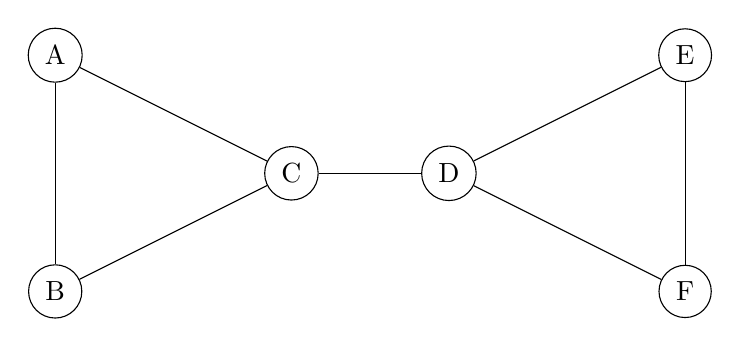
\begin{tikzpicture}
        \node[circle,draw] (A) at (0, 3) {A};
        \node[circle,draw] (B) at (0, 0) {B};
        \node[circle,draw] (C) at (3, 1.5) {C};
        \node[circle,draw] (D) at (5, 1.5) {D};
        \node[circle,draw] (E) at (8, 3) {E};
        \node[circle,draw] (F) at (8, 0) {F};
        
        \draw (A) -- (B);
        \draw (A) -- (C);
        \draw (B) -- (C);
        \draw (C) -- (D);
        \draw (D) -- (E);
        \draw (D) -- (F);
        \draw (E) -- (F);
    \end{tikzpicture}
\end{figure}

\subsubsection*{مقدار BC را برای راس \lr{C} به شکل زیر مشخص می‌کنیم.}

\begin{equation}
(A,B) = \sigma_{A,B} \rightarrow 1, (A,B) = \sigma_{A,B(C)} \rightarrow 0, (\sigma_{A,B(C)}/\sigma_{A,B}) = 0/1 \rightarrow 0
\end{equation}

\begin{equation}
(A,D) = \sigma_{A,D} \rightarrow 1, (A,D) = \sigma_{A,D(C)} \rightarrow 1, (\sigma_{A,D(C)}/\sigma_{A,D}) = 1/1 \rightarrow 1
\end{equation}

\begin{equation}
(A,E) = \sigma_{A,E} \rightarrow 1, (A,E) = \sigma_{A,E(C)} \rightarrow 1, (\sigma_{A,E(C)}/\sigma_{A,E}) = 1/1 \rightarrow 1
\end{equation}

\begin{equation}
(A,F) = \sigma_{A,F} \rightarrow 1, (A,F) = \sigma_{A,F(C)} \rightarrow 1, (\sigma_{A,F(C)}/\sigma_{A,F}) = 1/1 \rightarrow 1
\end{equation}

\begin{equation}
(B,D) = \sigma_{B,D} \rightarrow 1, (B,D) = \sigma_{B,D(C)} \rightarrow 1, (\sigma_{B,D(C)}/\sigma_{B,D}) = 1/1 \rightarrow 1
\end{equation}

\begin{equation}
(B,E) = \sigma_{B,E} \rightarrow 1, (B,E) = \sigma_{B,E(C)} \rightarrow 1, (\sigma_{B,E(C)}/\sigma_{B,E}) = 1/1 \rightarrow 1
\end{equation}

\begin{equation}
(B,F) = \sigma_{B,F} \rightarrow 1, (B,F) = \sigma_{B,F(C)} \rightarrow 1, (\sigma_{B,F(C)}/\sigma_{B,F}) = 1/1 \rightarrow 1
\end{equation}

\begin{equation}
(E,F) = \sigma_{E,F} \rightarrow 1, (E,F) = \sigma_{E,F(C)} \rightarrow 0, (\sigma_{E,F(C)}/\sigma_{B,F}) = 0/1 \rightarrow 0
\end{equation}

\begin{equation}
(D,E) = \sigma_{D,E} \rightarrow 1, (D,E) = \sigma_{D,E(C)} \rightarrow 0, (\sigma_{D,E(C)}/\sigma_{D,E}) = 0/1 \rightarrow 0
\end{equation}

مقدار \lr{Betweenness centrality} براساس راس \lr{C} برابر با ۶ است.

به دلیل آنکه \lr{C} و \lr{D} با یکدیگر در یک راستا و سطح گراف هستند پس مقدار راس
\lr{D} هم مانند راس \lr{C} برابر با ۶ می‌باشد.

تمامی گوشه‌های گراف مقدار \lr{BC} آنها برابر با ۰ می‌باشد.

\begin{figure}[H]
    \centering
    \includegraphics[width=0.7\textwidth]{images/betweenness_centrality_false.png}
    \caption{گراف \lr{Betweenness centrality}}
    \label{fig: bc_mst_off}
\end{figure}

از \lr{Degree} و \lr{BC} هر کدام از پروتئین‌ها را استفاده می‌کنیم که دو پارامتر
رنگ و اندازه را از طریق وزن یال‌ها بدست آوریم.

رنگ‌ها از بنفش پررنگ شروع می‌شود تا زرد روشن. هر چقدر یک پروتئین زرد‌تر باشد
درجه بیشتری را دارا می‌باشد. بزرگ‌ترین پروتئین بیشترین \lr{BC} را بین
پروتئین‌های دیگر دارد.

\subsection{نظریه \lr{Minimum Spanning Tree} \cite{enwiki:1213233694}}

گرافی است بدون حلقه، زیر مجموعه تمام لبه‌هایی که گره‌ها را با کمترین وزن ممکن به
یکدگیر متصل می‌کند.

\begin{figure}[H]
    \centering
    \includegraphics[width=0.9\textwidth]{images/betweenness_centrality_true.png}
    \caption{بهینه‌سازی گراف با \lr{mst}}
    \label{fig: bc_mst_on}
\end{figure}

\newpage
\bibliographystyle{plain-fa}
\bibliography{refs.bib}

\end{document}